\chapter[Production]{Production}
This chapter will explain the process of going from a theoretical design to actual implementation. First, the system will be simulated, and the results will be reviewed. Lastly, the process of producing the physical hardware will be discussed.
\section{Simulation}
During the synthesis phase of the project, it was decided that it would be a valuable learning tool to use the understanding gained from studying the materials and theory to come up with a SPICE model that can simulate the design. For simplicity, it would be beneficial to the simulation to use ideal components rather than complex physical models. This causes the circuit simulation to compute faster (because of less complex calculations) and causes the simulation to be easier to troubleshoot. The gate driver is replaced by a buffer without hysteresis and complementary output, and the power stage is replaced by a VCVS also called an E source in LTSpice. To streamline simulation efforts by using MATLAB for carrying out the necessary synthesis calculations and inputting those component values to the simulations in LTSpice, the script \autoref{lst:simulationLTspice.m} will export the component values to an external parameter file, import the parameters in LTspice and perform the simulation. The simulation output is imported automatically to MATLAB using the library ltspice2matlab \cite{ltspice2matlab} for post-processing and analysis. This improves workflow and makes it possible to compare various sets of parameters efficiently. \\
The transient simulations are performed for a length of \SI{600}{\micro\second} with a log delay of \SI{200}{\micro\second} to ensure a steady state. The input signal is configured with a DC component of $V_{\mathrm{DC}} = \SI{2.5}{\volt}$, AC component $v_{\mathrm{p-p}} = \SI{900}{\milli\volt}$ and frequency of $f_{\mathrm{in}} = \SI{10}{\kilo\hertz}$.

\subsection{Open Loop}
A simulation model based on the theory of each function can be seen implemented in LTSpiceXVII in the figure below:
\begin{figure}[H]
	\centering
	\includegraphics[width=0.9\textwidth,trim=5 260 5 260, clip]{0_Figures/Production/ltspice_sim_openloop.pdf}
	\caption{LTspice model of class-D amplifier using ideal components without feedback}
	\label{fig:ltspice_sim_openloop}
\end{figure}
Seen in \autoref{fig:ltspice_sim_openloop} is the circuit as described in the synthesis chapter, although with the gate driver circuit and power stage implemented with ideal components rather than complex SPICE component models. Upon simulating the circuit and analysing the following data is obtained:
\begin{figure}[htbp]
	\centering
	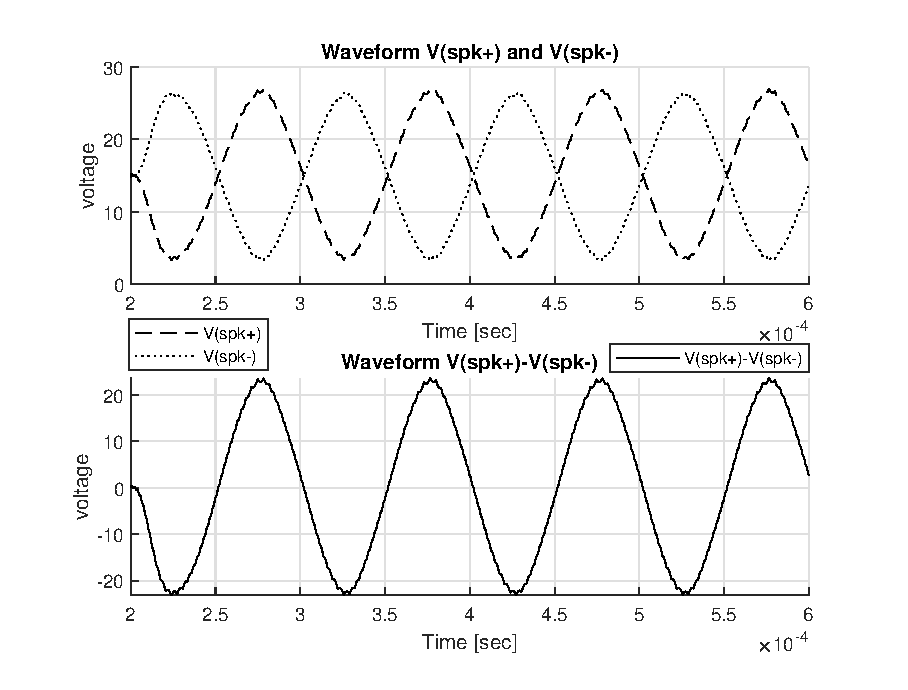
\includegraphics[width=0.9\textwidth]{Production/sim_openloop_output.eps}
	\caption{LTspice simulation output of openloop configuration}
	\label{fig:ltspice_sim_openloop_output}
\end{figure}
On \autoref{fig:ltspice_sim_openloop_output} the output of the open loop transient simulation from \autoref{fig:ltspice_sim_openloop} can be seen. Note that under the x-axis of the figure, it is zeroed at \SI{200}{\micro\second}. This is done to ensure a steady-state in the transient simulation. In the upper subfigure the two node voltages of the bridge-tied load can be seen as described in the LTspice model in \autoref{fig:ltspice_sim_openloop}. In the output signal on both subfigures some noticeable but minor output ripple can be seen. This is due to the reactive components characteristics in the output filter.

\begin{figure}[htbp]
	\begin{subfigure}[t]{0.5\textwidth}
		\centering
		\includegraphics[width=\linewidth]{Production/sim_open_fosc.eps}
		\subcaption{$f_{\mathrm{sw}}$ over $V_{\mathrm{in}}$}
		\label{fig:ltspice_aim_fosc}
	\end{subfigure}%
	\begin{subfigure}[t]{0.5\textwidth}
		\centering
		\includegraphics[width=\linewidth]{Production/sim_open_duty.eps}
		\subcaption{$D$ over $V_{\mathrm{in}}$}
		\label{fig:ltspice_aim_duty}
	\end{subfigure}
	\caption{Simulated $f_{\mathrm{sw}}$ and $D$ over DC values of $V_{\mathrm{in}}$ with zero amplitude}
	\label{fig:ltspice_aim}
\end{figure}
Seen in \autoref{fig:ltspice_aim} is the simulated AIM, plotted for $f_{\mathrm{sw}}$ in \Cref{fig:ltspice_aim_fosc} and $D$ in \Cref{fig:ltspice_aim_duty}. This is done with zero amplitude and a step parameter of DC input. It is noted that the switching frequency produces the expected curve according to the calculations. This varying switching frequency is a particular trait of the astable integrating modulator due to the non-linear behavior of the carrier waveform and the propagated phase delay of the self-oscillation. The duty cycle fits the theoretical model as seen in in \Cref{fig:modulator_duty_synth}.
%skriv om hvad der ses


\subsection{Closed Loop}
\begin{figure}[htbp]
	\centering
	\includegraphics[width=0.9\textwidth,trim=5 230 5 230, clip]{0_Figures/Production/ltspice_sim_regulator.pdf}
	\caption{LTspice model of class-D amplifier using ideal power stage switches with a control loop}
	\label{fig:ltspice_sim_closedloop}
\end{figure}
Seen in \autoref{fig:ltspice_sim_closedloop} is the circuit as described in its entirety. This includes the control loop with the LQR and PI controller feedback loop from the bridge-tied load.

\begin{figure}[htbp]
	\centering
	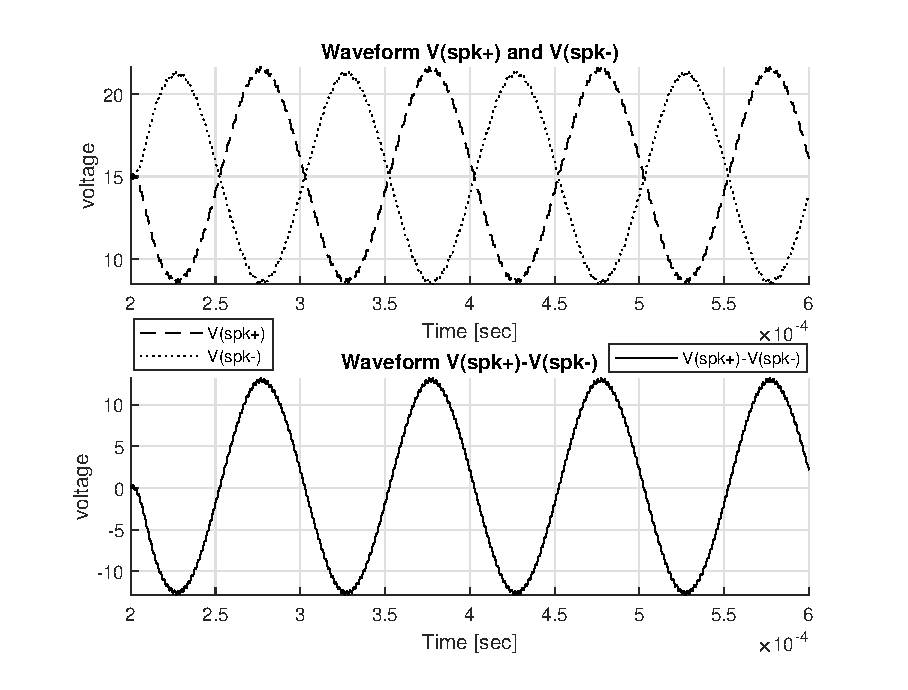
\includegraphics[width=0.9\textwidth]{Production/sim_closedloop_output.eps}
	\caption{LTspice simulation output of closed loop configuration}
	\label{fig:ltspice_sim_closedloop_output}
\end{figure}
The output from the closed loop simulation model can be seen in \autoref{fig:ltspice_sim_closedloop_output}. Note that under the x-axis of the figure, it is zeroed at \SI{200}{\micro\second}. This is undertaken to ensure a steady-state in the transient simulation. In the upper subfigure are the two voltage nodes on each side of the bridge-tied load and in the lower plot is the differential output signal. It is noted that the amplitude of the differential output signal is approximately half of the open loop configuration.
\clearpage
\section{Inductor design}
%TODO Skriv noget om spole vikling og kerne valg, etc. Referer til \autoref{lst:inductor_design2}
During the synthesis phase, a value for the output filter inductor was obtained. Now, an inductor design must be made with regards to core material, core size and wire gauge. Based on an initial proposal, it was decided to investigate between two options being MICROMETALS, Inc. toroid cores of the T80-2 and T94-2 variants. The choice being a relatively small core size that would adequately fit the PCB in a parallel mounting position, and a material '2'-type that holds necessary linear frequency characteristics. The inductor wire gauge was chosen fairly large to retain a modest number of turns and in turn causing the winding to be easier to do by hand.
Based on the datasheet \cite{micrometals} expressions, the calculations were made in MATLAB in accordance with \autoref{lst:inductor_design2}. The calculation showing that both options are valid choices in terms of not saturating the core and yielding the following results. \\
For T-80-2:
$$N = \SI{17}{\turns}$$
$$B = \SI{32}{\milli\tesla}$$
For T-94-2:
$$N = \SI{14.5}{\turns}$$
$$B = \SI{25}{\milli\tesla}$$
The T-80-2 was chosen because of its smaller core size and wound by hand using \SI{0.95}{\milli\meter} wire gauge from inventory. \\
\subsubsection{Measurement}
After winding the two coils, a validation of the coil specifications is needed. A lab test with a N4L PSM1735 frequency analyzer \cite{n4l_analyzer}, the following inductance over frequency was measured:
\begin{figure}[htbp]
	\centering
	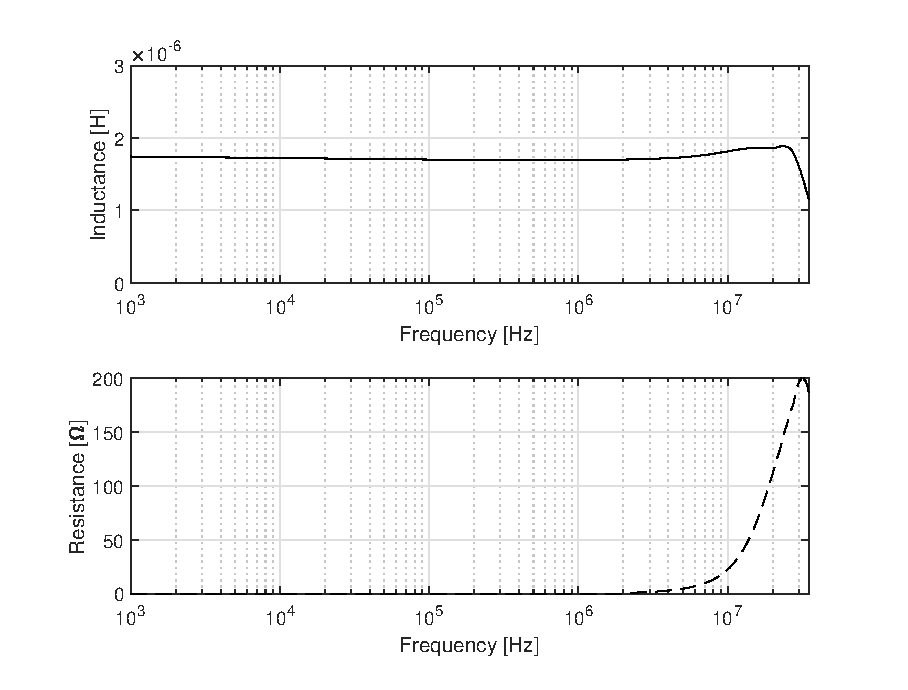
\includegraphics[width=0.9\textwidth]{Production/coil_measurement.eps}
	\caption{Inductor measurement over the frequency range \SIrange[scientific-notation = engineering]{1000}{35000000}{\hertz}}
	\label{fig:inductor_measurement}
\end{figure}
Seen in \autoref{fig:inductor_measurement}, is a measurement sweep with the wound inductor coil under test. The upper subfigureshows inductance over frequency, and measures reasonably the expected \SI{1.768}{\micro\henry} on the output filter inductor. relatively linearly until around \SI{10}{\mega\hertz} where there is a peak and then a drop-off in inductance. As this frequency is significantly higher than the switching frequency of the pulse signal it is acceptable. The lower subfigure describes the resistance over frequency and is also comparatively low until it reaches \SI{20}{\ohm} at \SI{10}{\mega\hertz}. This should give an idea of the amount of heat dissipation within the output filter inductors can be negligible on the frequency range of interest.

\subsection{Mounting method}
In the PCB design a through-hole mounting was decided in the original design. However, in the project a surface mount was decided. The problem with mounting the output filter inductors in the through-hole method is that it can cause the removal to be much more difficult as well as the protrusion of the conducting wires on the opposing side of the PCB can increase EMI in the sensitive circuitry.

\begin{figure}[htbp]
	\centering
	\begin{subfigure}[t]{0.5\textwidth}
		\centering
		

% Pattern Info
 
\tikzset{
pattern size/.store in=\mcSize, 
pattern size = 5pt,
pattern thickness/.store in=\mcThickness, 
pattern thickness = 0.3pt,
pattern radius/.store in=\mcRadius, 
pattern radius = 1pt}
\makeatletter
\pgfutil@ifundefined{pgf@pattern@name@_8hsyz2x1h}{
\pgfdeclarepatternformonly[\mcThickness,\mcSize]{_8hsyz2x1h}
{\pgfqpoint{-\mcThickness}{-\mcThickness}}
{\pgfpoint{\mcSize}{\mcSize}}
{\pgfpoint{\mcSize}{\mcSize}}
{
\pgfsetcolor{\tikz@pattern@color}
\pgfsetlinewidth{\mcThickness}
\pgfpathmoveto{\pgfpointorigin}
\pgfpathlineto{\pgfpoint{0}{\mcSize}}
\pgfusepath{stroke}
}}
\makeatother

% Pattern Info
 
\tikzset{
pattern size/.store in=\mcSize, 
pattern size = 5pt,
pattern thickness/.store in=\mcThickness, 
pattern thickness = 0.3pt,
pattern radius/.store in=\mcRadius, 
pattern radius = 1pt}
\makeatletter
\pgfutil@ifundefined{pgf@pattern@name@_k471tnbv3}{
\pgfdeclarepatternformonly[\mcThickness,\mcSize]{_k471tnbv3}
{\pgfqpoint{-\mcThickness}{-\mcThickness}}
{\pgfpoint{\mcSize}{\mcSize}}
{\pgfpoint{\mcSize}{\mcSize}}
{
\pgfsetcolor{\tikz@pattern@color}
\pgfsetlinewidth{\mcThickness}
\pgfpathmoveto{\pgfpointorigin}
\pgfpathlineto{\pgfpoint{0}{\mcSize}}
\pgfusepath{stroke}
}}
\makeatother
\tikzset{every picture/.style={line width=0.75pt}} %set default line width to 0.75pt        

\begin{tikzpicture}[x=0.75pt,y=0.75pt,yscale=-1,xscale=1]
%uncomment if require: \path (0,125); %set diagram left start at 0, and has height of 125

%Shape: Rectangle [id:dp18833028707967348] 
\draw  [color={rgb, 255:red, 0; green, 0; blue, 0 }  ,draw opacity=1 ] (10,92) -- (140,92) -- (140,102) -- (10,102) -- cycle ;
%Shape: Circle [id:dp7926791153140256] 
\draw  [fill={rgb, 255:red, 79; green, 107; blue, 63 }  ,fill opacity=1 ] (40,47) .. controls (40,27.67) and (55.67,12) .. (75,12) .. controls (94.33,12) and (110,27.67) .. (110,47) .. controls (110,66.33) and (94.33,82) .. (75,82) .. controls (55.67,82) and (40,66.33) .. (40,47) -- cycle ;
%Shape: Rectangle [id:dp9861901382755367] 
\draw  [pattern=_8hsyz2x1h,pattern size=2.325pt,pattern thickness=0.75pt,pattern radius=0pt, pattern color={rgb, 255:red, 0; green, 0; blue, 0}] (40,92) -- (50,92) -- (50,102) -- (40,102) -- cycle ;
%Shape: Rectangle [id:dp8283079391334511] 
\draw  [pattern=_k471tnbv3,pattern size=2.325pt,pattern thickness=0.75pt,pattern radius=0pt, pattern color={rgb, 255:red, 0; green, 0; blue, 0}] (100,92) -- (110,92) -- (110,102) -- (100,102) -- cycle ;
%Shape: Circle [id:dp9007499783674364] 
\draw  [fill={rgb, 255:red, 255; green, 255; blue, 255 }  ,fill opacity=1 ] (50,47) .. controls (50,33.19) and (61.19,22) .. (75,22) .. controls (88.81,22) and (100,33.19) .. (100,47) .. controls (100,60.81) and (88.81,72) .. (75,72) .. controls (61.19,72) and (50,60.81) .. (50,47) -- cycle ;
%Shape: Free Drawing [id:dp6271843413886811] 
\draw  [color={rgb, 255:red, 0; green, 0; blue, 0 }  ][line width=1.5] [line join = round][line cap = round] (42.5,71) .. controls (48.71,67.9) and (62.69,61.6) .. (51.5,56) ;
%Shape: Free Drawing [id:dp05242952437084436] 
\draw  [color={rgb, 255:red, 0; green, 0; blue, 0 }  ][line width=1.5] [line join = round][line cap = round] (38.5,49) .. controls (44.66,49) and (48.38,47.56) .. (53.5,45) ;
%Shape: Free Drawing [id:dp7113877869069425] 
\draw  [color={rgb, 255:red, 0; green, 0; blue, 0 }  ][line width=1.5] [line join = round][line cap = round] (46.5,26) .. controls (49.53,28.27) and (54.81,37.69) .. (59.5,33) ;
%Shape: Free Drawing [id:dp6598413365259324] 
\draw  [color={rgb, 255:red, 0; green, 0; blue, 0 }  ][line width=1.5] [line join = round][line cap = round] (67.5,13) .. controls (67.5,19.05) and (68.78,25) .. (75.5,25) ;
%Shape: Free Drawing [id:dp7040403620857618] 
\draw  [color={rgb, 255:red, 0; green, 0; blue, 0 }  ][line width=1.5] [line join = round][line cap = round] (98.5,21) .. controls (98.5,4.2) and (78.93,27.42) .. (85.5,31) .. controls (88.72,32.76) and (92.83,31) .. (96.5,31) ;
%Shape: Free Drawing [id:dp338560523548316] 
\draw  [color={rgb, 255:red, 0; green, 0; blue, 0 }  ][line width=1.5] [line join = round][line cap = round] (112.5,39) .. controls (115.5,39) and (106.45,38.45) .. (103.5,39) .. controls (98.49,39.94) and (91.8,46) .. (101.5,46) ;
%Shape: Free Drawing [id:dp25756137484802855] 
\draw  [color={rgb, 255:red, 0; green, 0; blue, 0 }  ][line width=1.5] [line join = round][line cap = round] (95.5,60) .. controls (95.5,58.05) and (93.62,57.76) .. (94.5,56) .. controls (99.41,46.17) and (109.5,58.62) .. (109.5,64) ;
%Shape: Free Drawing [id:dp5167102379219084] 
\draw  [color={rgb, 255:red, 0; green, 0; blue, 0 }  ][line width=1.5] [line join = round][line cap = round] (110.5,63) .. controls (110.5,65.33) and (110.79,67.68) .. (110.5,70) .. controls (110.32,71.45) and (106.64,73.34) .. (106.5,76) .. controls (105.89,87.32) and (106.5,98.67) .. (106.5,110) ;
%Shape: Free Drawing [id:dp9636921436425505] 
\draw  [color={rgb, 255:red, 0; green, 0; blue, 0 }  ][line width=1.5] [line join = round][line cap = round] (44.5,69) .. controls (40.67,74.75) and (44.14,78.9) .. (44.5,84) .. controls (45.09,92.31) and (44.5,100.67) .. (44.5,109) ;




\end{tikzpicture}

		\subcaption{Through-hole mounting}
		\label{fig:inductor_mount_thruhole}
	\end{subfigure}%
	\begin{subfigure}[t]{0.5\textwidth}
		\centering
		

% Pattern Info

\tikzset{
	pattern size/.store in=\mcSize, 
	pattern size = 5pt,
	pattern thickness/.store in=\mcThickness, 
	pattern thickness = 0.3pt,
	pattern radius/.store in=\mcRadius, 
	pattern radius = 1pt}
\makeatletter
\pgfutil@ifundefined{pgf@pattern@name@_loi3sd3p3}{
	\pgfdeclarepatternformonly[\mcThickness,\mcSize]{_loi3sd3p3}
	{\pgfqpoint{-\mcThickness}{-\mcThickness}}
	{\pgfpoint{\mcSize}{\mcSize}}
	{\pgfpoint{\mcSize}{\mcSize}}
	{
		\pgfsetcolor{\tikz@pattern@color}
		\pgfsetlinewidth{\mcThickness}
		\pgfpathmoveto{\pgfpointorigin}
		\pgfpathlineto{\pgfpoint{0}{\mcSize}}
		\pgfusepath{stroke}
}}
\makeatother

% Pattern Info

\tikzset{
	pattern size/.store in=\mcSize, 
	pattern size = 5pt,
	pattern thickness/.store in=\mcThickness, 
	pattern thickness = 0.3pt,
	pattern radius/.store in=\mcRadius, 
	pattern radius = 1pt}
\makeatletter
\pgfutil@ifundefined{pgf@pattern@name@_e59b6qrtq}{
	\pgfdeclarepatternformonly[\mcThickness,\mcSize]{_e59b6qrtq}
	{\pgfqpoint{-\mcThickness}{-\mcThickness}}
	{\pgfpoint{\mcSize}{\mcSize}}
	{\pgfpoint{\mcSize}{\mcSize}}
	{
		\pgfsetcolor{\tikz@pattern@color}
		\pgfsetlinewidth{\mcThickness}
		\pgfpathmoveto{\pgfpointorigin}
		\pgfpathlineto{\pgfpoint{0}{\mcSize}}
		\pgfusepath{stroke}
}}
\makeatother
\tikzset{every picture/.style={line width=0.75pt}} %set default line width to 0.75pt        

\begin{tikzpicture}[x=0.75pt,y=0.75pt,yscale=-1,xscale=1]
	%uncomment if require: \path (0,125); %set diagram left start at 0, and has height of 125
	
	%Shape: Rectangle [id:dp2009637706126184] 
	\draw  [color={rgb, 255:red, 0; green, 0; blue, 0 }  ,draw opacity=1 ] (10,90) -- (140,90) -- (140,100) -- (10,100) -- cycle ;
	%Shape: Circle [id:dp1038951998619202] 
	\draw  [fill={rgb, 255:red, 79; green, 107; blue, 63 }  ,fill opacity=1 ] (40,45) .. controls (40,25.67) and (55.67,10) .. (75,10) .. controls (94.33,10) and (110,25.67) .. (110,45) .. controls (110,64.33) and (94.33,80) .. (75,80) .. controls (55.67,80) and (40,64.33) .. (40,45) -- cycle ;
	%Shape: Rectangle [id:dp645799702370889] 
	\draw  [pattern=_loi3sd3p3,pattern size=2.325pt,pattern thickness=0.75pt,pattern radius=0pt, pattern color={rgb, 255:red, 0; green, 0; blue, 0}] (40,90) -- (50,90) -- (50,100) -- (40,100) -- cycle ;
	%Shape: Rectangle [id:dp7924832651254976] 
	\draw  [pattern=_e59b6qrtq,pattern size=2.325pt,pattern thickness=0.75pt,pattern radius=0pt, pattern color={rgb, 255:red, 0; green, 0; blue, 0}] (100,90) -- (110,90) -- (110,100) -- (100,100) -- cycle ;
	%Shape: Circle [id:dp17475143217548772] 
	\draw  [fill={rgb, 255:red, 255; green, 255; blue, 255 }  ,fill opacity=1 ] (50,45) .. controls (50,31.19) and (61.19,20) .. (75,20) .. controls (88.81,20) and (100,31.19) .. (100,45) .. controls (100,58.81) and (88.81,70) .. (75,70) .. controls (61.19,70) and (50,58.81) .. (50,45) -- cycle ;
	%Shape: Free Drawing [id:dp0066542513246226065] 
	\draw  [color={rgb, 255:red, 0; green, 0; blue, 0 }  ][line width=1.5] [line join = round][line cap = round] (42.5,69) .. controls (48.71,65.9) and (62.69,59.6) .. (51.5,54) ;
	%Shape: Free Drawing [id:dp02794267711535947] 
	\draw  [color={rgb, 255:red, 0; green, 0; blue, 0 }  ][line width=1.5] [line join = round][line cap = round] (38.5,47) .. controls (44.66,47) and (48.38,45.56) .. (53.5,43) ;
	%Shape: Free Drawing [id:dp5943567299775048] 
	\draw  [color={rgb, 255:red, 0; green, 0; blue, 0 }  ][line width=1.5] [line join = round][line cap = round] (46.5,24) .. controls (49.53,26.27) and (54.81,35.69) .. (59.5,31) ;
	%Shape: Free Drawing [id:dp10842246038623493] 
	\draw  [color={rgb, 255:red, 0; green, 0; blue, 0 }  ][line width=1.5] [line join = round][line cap = round] (67.5,11) .. controls (67.5,17.05) and (68.78,23) .. (75.5,23) ;
	%Shape: Free Drawing [id:dp3973786711513443] 
	\draw  [color={rgb, 255:red, 0; green, 0; blue, 0 }  ][line width=1.5] [line join = round][line cap = round] (98.5,19) .. controls (98.5,2.2) and (78.93,25.42) .. (85.5,29) .. controls (88.72,30.76) and (92.83,29) .. (96.5,29) ;
	%Shape: Free Drawing [id:dp9304280952996944] 
	\draw  [color={rgb, 255:red, 0; green, 0; blue, 0 }  ][line width=1.5] [line join = round][line cap = round] (112.5,37) .. controls (115.5,37) and (106.45,36.45) .. (103.5,37) .. controls (98.49,37.94) and (91.8,44) .. (101.5,44) ;
	%Shape: Free Drawing [id:dp6543954815936195] 
	\draw  [color={rgb, 255:red, 0; green, 0; blue, 0 }  ][line width=1.5] [line join = round][line cap = round] (95.5,58) .. controls (95.5,56.05) and (93.62,55.76) .. (94.5,54) .. controls (99.41,44.17) and (109.5,56.62) .. (109.5,62) ;
	%Shape: Free Drawing [id:dp6148483141653001] 
	\draw  [color={rgb, 255:red, 0; green, 0; blue, 0 }  ][line width=1.5] [line join = round][line cap = round] (42.5,68) .. controls (41.45,69.05) and (36.8,71.09) .. (36.5,72) .. controls (35.69,74.43) and (39.4,85.83) .. (40.5,86) .. controls (45.11,86.71) and (49.83,86) .. (54.5,86) ;
	%Shape: Free Drawing [id:dp8979898934658102] 
	\draw  [color={rgb, 255:red, 0; green, 0; blue, 0 }  ][line width=1.5] [line join = round][line cap = round] (110.5,60) .. controls (110.5,68) and (121.72,85.81) .. (107.5,88) .. controls (103.53,88.61) and (99.09,88.8) .. (95.5,87) ;
	%Shape: Free Drawing [id:dp6437402351035637] 
	\draw  [color={rgb, 255:red, 0; green, 0; blue, 0 }  ][line width=1.5] [line join = round][line cap = round] (37.5,88) .. controls (42.68,89.3) and (48.17,89.44) .. (53.5,89) .. controls (58.49,88.58) and (43.51,88) .. (38.5,88) .. controls (37.17,88) and (41.18,88.22) .. (42.5,88) .. controls (44.23,87.71) and (49.5,84.9) .. (49.5,87) ;
	%Shape: Free Drawing [id:dp07779661964495088] 
	\draw  [color={rgb, 255:red, 0; green, 0; blue, 0 }  ][line width=1.5] [line join = round][line cap = round] (100.5,89) .. controls (103.83,88.67) and (107.25,88.81) .. (110.5,88) .. controls (111.67,87.71) and (114.7,86) .. (113.5,86) .. controls (113.48,86) and (102.21,87.98) .. (102.5,88) .. controls (106.49,88.33) and (110.5,88) .. (114.5,88) ;
	
	
	
	
\end{tikzpicture}

		\subcaption{Surface mounting}
		\label{fig:inductor_mount_surface}
	\end{subfigure}
	\caption{Inductor mounting sketch, not to scale}
	\label{fig:inductor_mounting}
\end{figure}

Seen in \autoref{fig:inductor_mounting} are two possible ways to mount the output filter inductors. In \Cref{fig:inductor_mount_thruhole} the two conductive wires of the inductor are inserted through the Via on the PCB and soldered on the opposing end. In \Cref{fig:inductor_mount_surface} the two wires are bent and soldered to the Via on the same side as the inductor. In this project the primary benefit of this mounting method is that it is desired to be able to test different inductors and it considers the possibility to remove the coil a requirement. A through-hole mounting is not ideal because the increased thermal connection becomes excessively large and the introduced heat on the copper by the soldering iron is dissipated into other areas of the PCB. Therefore, some heat restriction is required. This is knowledge that was acquired experimentally during the mounting process.

\section{Printed Circuit Board}
This section will explain the process of manufacturing the physical PCBs for the class-D amplifier. The layout file from \cite{nagy_special_course} was used in this project. It is comprised of two PCBs. The first part handles the IO and in addition has the input filter, preamp and PI controller. The other PCB includes the modulation, power stage, output filter and regulation subcircuit. \\

\subsection{Input-Output Printed Circuit Board}
Refer to \autoref{fig:altium_layout_io_board} for the layout of the IO PCB.
\begin{figure}[htbp]
	\centering
	\includegraphics[width=0.9\textwidth,trim=0 175 0 175, clip]{0_Figures/Production/Control_PCB.pdf}
	\caption{Layout of IO PCB}
	\label{fig:altium_layout_io_board}
\end{figure}
\subsection{Amplifier Printed Circuit Board}
Refer to \autoref{fig:altium_layout_power_stage} for the Amplifier PCB.
\begin{figure}[htbp]
	\centering
	\includegraphics[width=0.6\textwidth,trim=60 0 60 40, clip]{0_Figures/Production/Power_Stage.pdf}
	\caption{Layout of Amplifier PCB}
	\label{fig:altium_layout_power_stage}
\end{figure}

\subsection{Methodology}

\begin{figure}[htbp]
	\centering
	\tcbox{\includegraphics[width=0.9\textwidth]{Production/amplifier_after_soldering.jpg}}
	\caption{Amplifier after solder work, without output filter inductors}
	\label{fig:amp_solder_no_coils}
\end{figure}
Seen in figure \autoref{fig:amp_solder_no_coils} are the two amplifier PCBs. The upper PCB is the IO, preamplifier, input filter and PI regulator. The lower PCB is amplifier.
The implementation is a 4-layer PCB design in Altium Designer and was manufactured professionally and sent to DTU without components. During production of the PCBs, a 63Sn/37Pb solder paste was added and SMD components were placed unto the PCB. Next the PCBs were placed in a reflow oven on the appropriate reflow cycle in accordance with the solder paste datasheet. Finally, the PCBs were inspected, cleaned and faulty soldering was corrected and through-hole components were soldered by hand. \\
During the production phase, some modifications were made to the original specification due to various circumstances like alternative inventory, better component choice, etc. A table with only the modifications to the BOM can be in \autoref{tab:bom_mod}.
\begin{table}[htbp]
	\adjustbox{max width=\textwidth}{%
	\centering
	\begin{tabular}{@{}llllll@{}}
		\toprule
		\textbf{Circuit} & \textbf{Component} & \textbf{Value} & \textbf{Footprint} & \textbf{Rating} & \textbf{Reason} \\ \midrule
		IO & C2,C3 & 120n & 0603 & X7R16V & 100n: No inventory \\
		IO & C4,C9,C10,C11 & 100n$\parallel$1u & 0603 & X7R16V & 120n: Improvement \\
		IO & C5 & 1u & 0603 & X7R50V & X5R6.3V: No inventory \\
		IO & C15 & 1.5n & 0603 & X7R16V & NC: Added \\
		IO & C8 & 1000u & RAD-0.3in & 63Vdc & 1500u: No inventory \\
		IO & R4,R7 & 3.01k & 0603 & 1\% & 4.75k: Improvement \\
		IO & R8 & 475 & 0603 & 1\% & 2.49k: Improvement \\
		Power stage & C11,C19 & 120n & 0603 & X7R16V & 100n: No inventory \\
		Power stage & C1,C15 & 22n$\parallel$1u & 0603 & X7R50V & 120n: Improvement \\
		Power stage & D1,D2 & Diode & NA & 75V 0.25A & 85V 0.25A: No inventory \\
		AIM+reg & C18,C20,C27, & 120n & 0603 & X7R16V & 100n: No inventory \\
		AIM+reg & C28,C29,C30,C31 & 120n & 0603 & X7R16V & 100n: No inventory \\
		AIM+reg & C8 & 120n & 0603 & X7R16V & Implement \\
		AIM+reg & RA1 & 2.21k & 0603 & 1\% & 2.2k: No inventory \\
		\bottomrule
	\end{tabular}}
	\caption{Modifications to the Bill of Materials}
	\label{tab:bom_mod}
\end{table}
% Skriv om PCB mods fra Søren - ind i ovenstående tabel
%IO BOARD
%Skift C4 til 100 nF || 1 uF
%Skift R4 og R7 til 3.01k
%Skift R8 til 475 ohm
%C9, C10, C11: 100 nF || 1 uF

%AMP
%Skift C1 og C15 til 22 nF + 1 uF (X7R 50 V)}
In the table with modifications to the BOM in conjunction with \autoref{tab:bom}, a comprehensive list of the amplifier components and their values are found. In the modification list, some components were experimentally improved in accordance with the further analysis.

\subsection{Remarks}
After the circuits were produced, components were soldered to the PCB as described in the previous section, initial inspections revealed some cross-connections due to imperfections in the soldering process. Therefore, manual corrections had to be done on the reflow process. Following the corrections, under visual inspection the PCBs appeared to be in a suitable condition. Some DMM measurements on the Amplifier PCB were performed to verify proper connections between ICs and the copper pads. This indicated adequate solder work ready for conclusive analysis.